\chapter{绪论}
\section{课题来源与意义}
近几年来,随着互联网(Internet)的兴起和发展,互联网上积累的数据呈现急剧膨胀的态势。根据国际数据信息公司\footnote{https://www.idc.com/}(International Data Corporation,IDC)的统计和预测,2018~年全球网络累积的数据量已经达到~1.8~ZB,预计到~2025~年全球网站数据累积总量还将增长约~50~倍。
随着这类无标注的文本和图像数据(Unlabeled Data)的大量涌现,如何利用现有的机器学习算法(Machine Learning),从这类无标注数据中学习内在规律并提取出有用的信息已经成了一个重要的挑战~\upcite{王建翔2017面向可读性评估的词向量技术研究及实现}。
自从2006 年以~Geoffrey Hinton~为代表的学者们提出深度学习(Deep Learning,DL)~\upcite{hinton2006reducing}理念以来,这一新的思路为解决如何利用爆炸的数据量,以提取有效知识带来了新的前景。
在这之后的发展中,基于神经网络(Neural Network,NN)的表示学习技术(Representation Learning)开始快速发展并拓展到相关研究领域中。
尤其在图像分类(Image Classification)、语音自动识别(Automatic Speech Recognition,ASR)~\upcite{DBLP:journals/taslp/WangW16}和神经机器翻译(Neural Machine Translation,NMT)~\upcite{bahdanau2014neural}等多个任务上,基于深度模型的方法在精确度和效率上远远超过了基于特征提取(Feature Extraction)的传统方法。

随着应用领域的拓展,深度学习技术逐渐在自然语言处理中(Natural Language Processing,NLP)得到广泛应用。 例如,蒙特利尔大学教授 Yousha Bengio 提出用神经网络来训练语言模型(Language Model,LM),并对模型中的各个结构细节进行了相关探索~\upcite{DBLP:conf/nips/BengioDV00}。因为模型的输入维度是固定的~N~个单词的词向量而不是动态长度的序列,所以该方法不能有效处理单词的长距离单词依赖问题(Long Term Dependency)。
在后续的工作中,其学生~Tomas Mikolov~针对这个问题提出了采用循环神经网络(Recurrent Neural Network, RNN)~\upcite{DBLP:journals/cogsci/Elman90}对上下文信息作为建模策略的方法,并逐步将该理论进行了拓展和简化\upcite{DBLP:conf/interspeech/MikolovKBCK10}。
循环神经网络主要特点是能够记忆该单词之前的所有单词的信息,即所谓的全局上下文信息(Global Context),用来预测下一个单词出现的对数概率分布。
因为RNN模型在训练过程中学习到了已经出现的单词信息,句子的长距离依赖关系可以被学习到,所以该方法在建模理论上克服了最初的神经网络语言模型的无法利用语句长距离上下文依赖的缺点。
另外,在模型训练的过程中,语义相似的单词将被映射到的同一低维子空间中,满足了单词语义相似(Semantic Similarity)的要求。相比统计语言模型(Statistical Language Model)领域中的N-gram模型,他不需要平滑技术(Smoothing Technology)来对文本中出现次数少的单词做处理。
到目前为止,RNN~模型已经演变出各种结构,应用在非常多的文本任务上面,并且都能取得了较为满意的结果。

由于循环网络的计算时间与句子的平均长度正相关,所以基于~RNN~建模的算法计算时间都很大,需要更长的计算时间收敛。同时,我们需要看到最简单的~RNN~模型所使用的参数数量是神经网络模型的两倍多,这也意味着~RNN~模型需要占用更大的内存空间和耗更多的计算资源,导致其无法广泛应用到现实场景中去。
在文献~\cite{DBLP:conf/icassp/MikolovKBCK11}~中,Tomas Mikolov~提出了多种优化策略来消除该模型的缺点,例如:缩短模型求导步数、对词表(Vocabulary)做分解~\upcite{DBLP:journals/coling/BrownPdLM92}等策略,这些计算策略能保证模型的计算精度,同时有效提高~RNN~网络的运算效率。

\section{国内外研究现状}
语言模型可以用来估算一段序列组合的可能性,该模型在机器翻译(Machine Translation)、语音识别(Speech Recognition)等任务上都有着极为重要的作用。语言模型具有漫长发展历史~\upcite{宗成庆2013统计自然语言处理},我们可以划分为两个主要阶段:统计语言模型(Statistical Language Model)和神经网络语言模型(Neural Language Model)。
其中,统计模型指代的是~N-gram~语言模型,而随着深度学习的爆发,各种神经网络语言模型变体被提出并占据了主导地位。我们接下来会对这两个演化阶段所涉及的算法进行介绍。

\subsection{N-gram 语言模型}
首先介绍传统~N-gram~语言模型,该算法属于典型的基于稀疏表示(Sparse Representation)的语言模型,因为一个单词表示方式是独热表示(One-Hot Representation)。该传统模型的意义不仅是提供了一种文本建模策略,而且定义了如何评价语言模型的优劣,并且定义了语言模型所涉及的相关拓展方向。

接下来给出~N-gram~统计语言模型的形式化定义。假设给定一个长度为~$m$~的单词字符串,$w_1$~到~$w_m$~依次表示这段文本中的各个单词,我们需要求解该序列的概率分布~$p(w_1,\cdots,w_m)$,以表示该字符串存在或者出现的可能性。在求解过程中,我们通常使用链式法则(Chain Rules)将求解整个序列的概率分解成计算单个单词的条件概率,如下形式:
\begin{equation}
\label{equ:lm}
p(w_1,\cdots,w_m) =p(w_1)\prod_{t=1}^{m}p(w_t|w_1,\cdots,w_{t-1})
\end{equation}
在实际求解过程中,如果文本的长度较长,公式~(\ref{equ:lm})~中右部~$p(w_t | w_1,w_2,\cdots,w_{t-1}) $ 的估计误差会相当大。因此~N~元模型(N-gram Model)和相应的平滑技术被提出,用于估算条件概率和减少概率估计误差。需要注意的是,单词距离大于~$N$~单词会被直接忽略,该模型可以写成如下形式:
\begin{equation}
\label{equ:approx}
p(w_t | w_1,w_2,\cdots,w_{t-1})  \approx p(w_t | w_{t-(n-1)},\cdots,w_{t-1})
\end{equation}
若~$N=1$~时,此时称为一元模型(Uni-gram Model),公式~(\ref{equ:approx})~将会退化成~$p(w_i),i\in [1,N-1]$.此时,整个句子的概率计算公式为:~$p(w_1,\cdots,w_m) = p(w_1)\cdots p(w_m)$。
从这个退化的公式中可以得知:在一元模型中,整个字符串的概率是出现的各个单词词频概率的乘积,它直接丢失了文本词组之间的顺序信息。当~$N=2$~时,称为二元模型(Bi-gram Model),公式~(\ref{equ:approx})~将会退化为 $p(w_t|w_{t-1})$。除此之外,还有~$N=3$~时的三元模型(Tri-gram model),使用~$p(w_t |w_{t-2},w_{t-1})$ 作为近似概率分布。除了一元模型外,二元模型、三元模型和后续的~N-gram~模型均可以保留一定的词序信息。

传统统计方法采用单词或者~N~元组的词频来作为~N~元组的概率计算方法,该方法简单有效且能满足线上负载的计算需求。但随着~N~的增大,模型的参数呈现指数爆炸式增长并且概率计算复杂度也相应上升。目前在线存储的~9~元模型(Google N-gram Viewer)\footnote{https://books.google.com/ngrams}已经达到了计算机存储和数据读取的极限。


神经网络语言模型的建模思路源于~N-gram~模型,主要解决的问题是如何对文本的上下文信息进行建模。历史上提出的模型可以主要分为:传统前向传递神经网络(Feed Forward Neural Network,FFNN)、双线性模型(Bilinear Model)以及循环神经网络(Recurrent Neural Network,RNN)等。 以下我们将对这三种主要的建模方案进行探讨。


\subsection{前馈神经网络语言模型}

由于神经网络对参数进行高度共享,因此对低频单词具有天然的平滑能力。这里所指的神经网络语言模型(Neural Probabilistic Language Model,NPLM) ,最早由~Bengio~等人在~2001~年提出~\upcite{DBLP:conf/nips/BengioDV00}, 近几年来学者开始展开这方面的研究并取得一系列成果,如~\cite{DBLP:conf/acl/BaroniDK14,DBLP:journals/sigkdd/BellK07,DBLP:journals/pami/BengioCV13,DBLP:journals/tnn/BengioSF94}~。
\begin{figure}
  \centering
  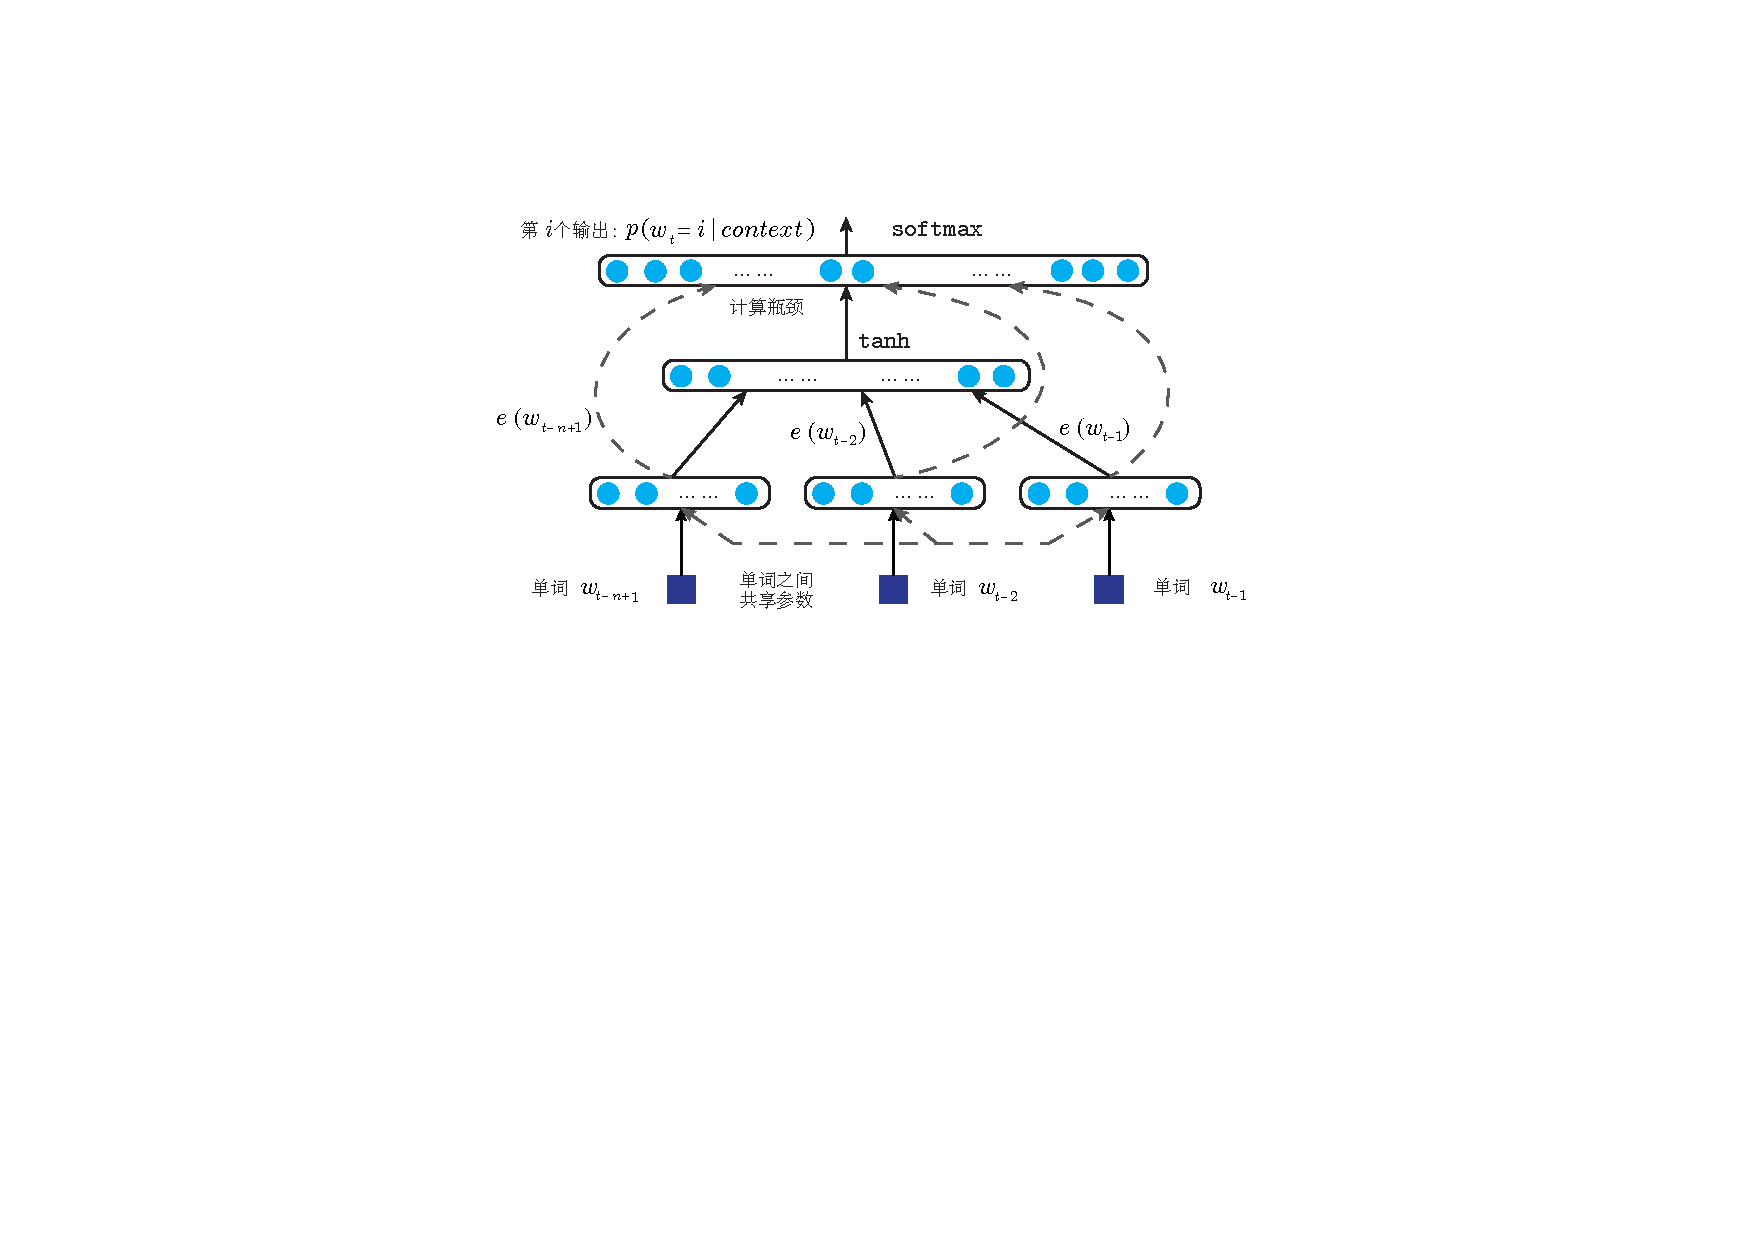
\includegraphics[width=.85\linewidth]{./figures/nplm.pdf}
  \caption{前馈神经网络语言模型}\label{fig:nplm}
\end{figure}

具体而言,NPLM通过一个多层感知网络(Multi-Layer Perceptron,MLP)来计算公式~(\ref{equ:approx})~中的概率。如图~\ref{fig:nplm}所示,输入层(Input Layer)用于表征前~$N$~个单词的高维分布;隐藏层(Hidden Layer)表征单词的上下文信息;最后的输出预测层(Output Layer)用于预测下一时刻的单词概率分布。为了解决~$N$~过大所带来的数据稀疏问题,Bengio~等人提出拼接(Concatenation)前~$N$~词的词向量作为输入,如下所示:
\begin{equation}\label{equ:we}
  x = [e(w_{t-(n-1)}), \cdots , e(w_{t-2}), e{(w_{t-1})}]
\end{equation}
模型的隐藏层~$h$~和输出层~$y$~可以依照下面的公式计算获得:
\begin{equation}\label{equ:nplm}
\begin{split}
h =& \tanh(Hx+b) \\
y =&Wx + Uh +b'
\end{split}
\end{equation}
其中参数矩阵~$H,W,U$~指代层与层之间连接的权重~\upcite{赵林2007一种新的基于结构的神经网络规则抽取方法},参数向量~$b,b'$~均为模型的偏置项(Bias Term)。如果存在~$W$,那么模型能直接学习到一个线性模型,需要训练的时间将会减半;如果不存在~$W$,模型将学习到非线性的网络从而具有更好的泛化性(Generalization)。因此在后续工作中,很少有使用输入层到输出层直连边的工作(即不存在~$W$~矩阵),下文我们也忽略这一种直连的操作。假设不考虑~$W$~矩阵,整个模型计算量最大的部分就是从隐藏层到输出层的矩阵运算~$U\times h$,后续的模型均有对这一矩阵乘法计算做优化。

\subsection{对数双线性语言模型}
2007 年,Mnih~和~Hinton~在神经网络语言模型(NPLM)的基础上提出了对数双线性语言模型(Log-Bilinear Language Model,LBL)~\upcite{DBLP:conf/icml/MnihH07}。其中~LBL~的模型结构是一个对数双线性网络结构,而~NPLM~的结构中不包含双线性结构,仅仅是简单的前馈网络。具体来讲,LBL~模型的代价函数为:
\begin{equation}
\label{equ:lbl}
\begin{split}
   &c=\sum_{i=1}^{n-1}{U_i e({w_i})}, \\
   &p(w_t=w|w_{1:t-1})=\frac{\exp(c^\top e(w))}{\sum_j{\exp(c^\top e(w_j))}}
\end{split}
\end{equation}
其中~$c$~代表了语言模型的上下文信息,$U_i$~指代的是对应单词词向量的权重。然后基于上下文信息表示~$c$~和目标词汇表中所有单词~$e(w),w\in \mathcal{V}$~的表示之间的相似度来计算下一个单词的可能的概率分布。

公式~(\ref{equ:lbl})~所描述LBL模型的代价函数与公式~(\ref{equ:nplm})~所描述~NPLM~模型的代价函数的主要区别包括:1) LBL~模型不包含非线性的激活函数~$\tanh$,而由于~NPLM~是非线性的神经网络结构,激活函数~$\tanh$~必不可少;2) LBL~模型中只有一份词向量~$e$,无论一个词是作为上下文还是作为目标词,使用的是同一份词向量,然而~NPLM~模型在输入端和预测端都有词向量矩阵,具有两份不同分布的词向量~$e$。其中第二个差一点只在最初提出的~LBL~模型中存在,后续的改进工作均不包含这一特点。

后续研究中,Mnih~等人以~LBL~模型为基础,并对其中存在缺点做了一系列改进工作,陆续提出了逆向量语言模型(inverse vector LBL,ivLBL)~\upcite{DBLP:conf/nips/MnihK13}和层次对数双线性语言模型(Hierarchical LBL,HLBL)~\upcite{DBLP:conf/icml/MnihT12}。

\subsection{循环神经网络语言模型}
对于循环神经网络来说,它能直接对公式~(\ref{equ:lm})~中的序列概率~$p(w_t | w_1,w_2,\cdots,w_{t-1})$~进行建模,而不需要使用公式~(\ref{equ:approx})~对其进行简化估计~\upcite{mikolov2012statistical,DBLP:conf/interspeech/MikolovKBCK10} 。RNNLM 模型结构如图~\ref{fig:rnnlm}~所示,它的核心方法在于其隐藏层的计算公式:
\begin{equation}
\label{equ:rnn}
  h_t \leftarrow  \phi(e(w_t) + U h_{t-1} +b),
\end{equation}
其中~$\phi$~为非线性激活函数。在上述公式中,$h_t$~表示文本中第~$t$~个词~$w_t$~所对应的隐藏层输出,由词向量 $e(w_t)$ 以及上一步的隐藏层输出~$h_{t -1}$~计算得到。隐藏层的初始状态为~$h_0$,随着模型逐个读入单词:$w_1,w_2,\cdots$, 根据公式~(\ref{equ:rnn})~逐步计算隐藏层并输出:$h_1,h_2,\cdots$ 。通过这种自身迭代更新方式,计算~$h_t$~时囊括了此前所有的信息~$w_1,w_2,\cdots,w_{t-1}$。最后,NPLM~模型和RNNLM 模型理论上能学习到更丰富、更长距离的知识,也有更大的潜力达到更好的效果。最后,RNNLM 模型的输出层与NPLM 模型的输出层都采用softmax算法,在该部分上两者是一致的。

\begin{figure}
  \centering
  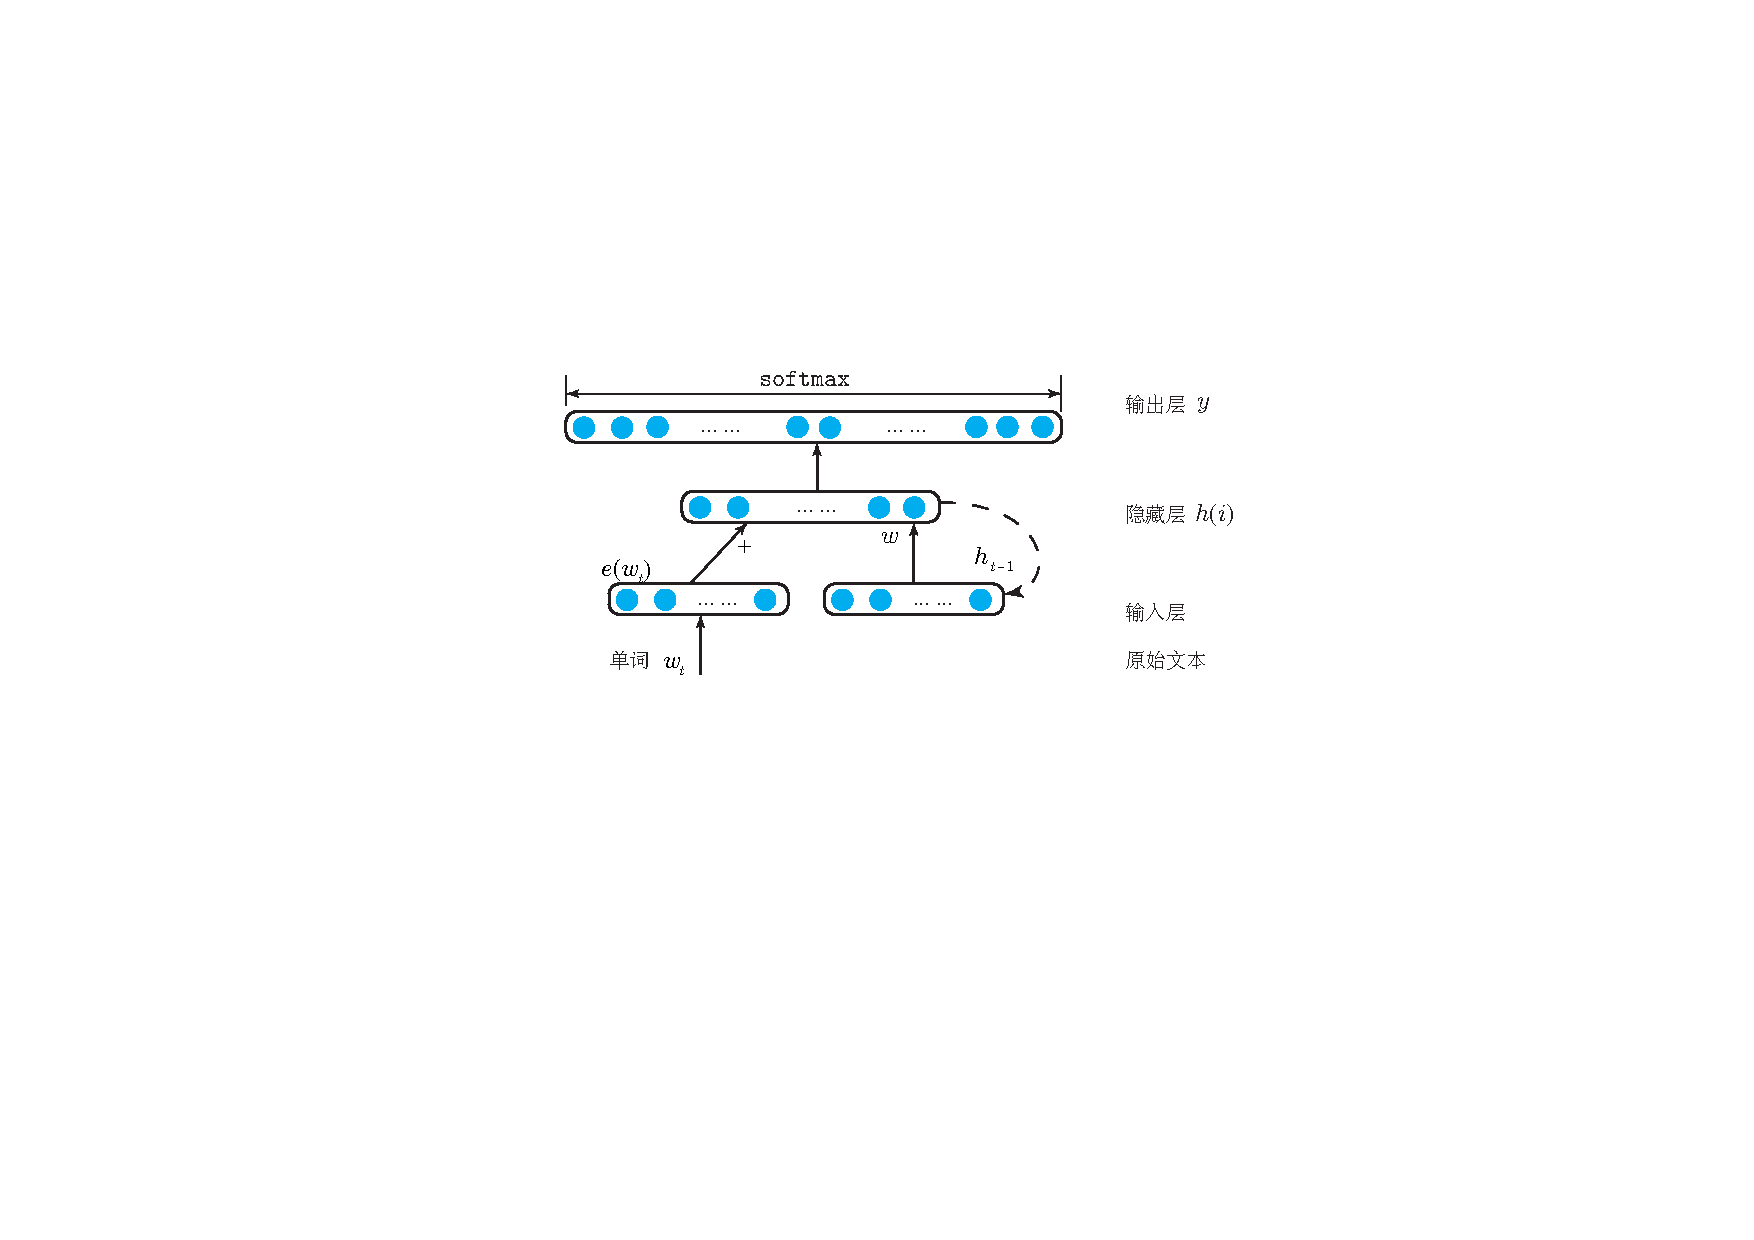
\includegraphics[width=.8\linewidth]{./figures/rnnlm.pdf}
  \caption{循环神经网络结构图}\label{fig:rnnlm}
\end{figure}

除了上述两种经典的建模方法,近几年研究者提出可以使用带有门限机制(Gating)的循环网络来防止模型的求导过程中导数趋近于~0~所带来的问题,例如长短记忆网络(Long Short-Term Memory,LSTM), 门限记忆节点(Gated Recurrent Unit,GRU)和其他网络。


\section{论文研究内容}
在历史文献当中,源词和目标词分别被称为模型的输入和输出。源词通常可以用分布式表示(Distributed Representation)来表示,称为输入词嵌入(Word Embedding),通常在大规模语料上使用连续词袋模型(CBoW)、跳跃单词模型(Skipgram)或者~Fasttext~模型来训练。
而这几种模型均起源于语言建模任务,并且考虑到实际运算的效率而去除了部分冗余结构。
另外,输出端的词表通常表示为单词索引(Indexing)或~$1-K$~编码,并且可以与~softmax~概率函数直接关联。

在语言模型研究领域中,大词表问题是目前理论应用到实际过程中必须要克服的问题,我们当然可以通过配置高性能服务器来缓解该计算瓶颈。一旦应用到较大规模的数据集上,即使是目前最好的中央处理器(CPU)或者通用计算图形处理器(GPGPU),仍然需要数周时间才能训练完善。因此,在保证原有模型的准确率和精度的前提下,如何提高模型的训练速度是本文主要讨论和研究的内容。为此我们考察了两个主要的研究目标:上下文信息建模效率和精度对比、大词表问题的优化和研究。

针对大词表问题的优化,目前主要采用的方案有以下几种:一种是采用子词(Subword-level)或者字符级别的词(Character-level)来直接缩小词表大小;一种是通过采样技术(Sampling-based Approximation)来减少必要的训练时间;另一种是通过基于分类的多元分类(class-based Hierarchical Softmax,cHSM)和采用基于树模型的多层二元分类模型(tree-based Hierarchical Softmax,tHSM)来加速模型。

本论文考虑了层次概率模型所存在的一些问题,并提出相应的解决策略。首先,我们提出了一个在分层结构上建模参数的单词编码方案,推导出紧凑的代价函数及其梯度。同时考虑到类或树上的单词分布对其性能有很大的影响,我们运用文本的统计,句法和语义知识来初始化其参差结构,以达到稳定的计算精度。同时在推理过程中,我们考虑了两种不同的推理情况:句子打分和文本排序,并提出了对应的优化策略。
\section{论文的组织结构}
\textbf{第一章:}``绪论'',主要介绍了本论文的研究背景和意义,另外简要说明了语言模型的发展历史以及本文的主要工作,并对本文的组织架构进行了说明。

\textbf{第二章:}``相关技术介绍'',对历史上的各个学术分支在语言模型的任务上的相关工作进行了介绍。

\textbf{第三章:}``树状层次概率模型'',介绍了基于二叉树的层次概率模型,并与传统树状模型做了理论层面的比较。同时还研究了在推理测试阶段,二叉树层次概率模型应用的贪心策略,以保证实际测试结果性能和效率。

\textbf{第四章:}``类别层次概率模型'',介绍基于分类的层次概率模型,并分析了词表非均匀划分所产生的后果,进而探讨了类别不均匀问题所带来的影响以及相关解决策略。最后探讨了在测试阶段,语言模型的任务需求和分类层次概率模型相应的解决算法。

\textbf{第五章:}``语言建模实验及结果分析'',实证研究了本论文提出的层次概率模型的实际效果,并和其他算法在各个指标维度上进行了比较和分析。

最后结论部分,总结了全论文的贡献和工作,并提出了未来的工作方向,同时撰写了结束语。



